\documentclass[12pt]{report}

% Mise en page
\textwidth 16cm
\textheight 23cm 
\topmargin -2 cm 
\oddsidemargin 0cm 
\evensidemargin 0cm
\renewcommand{\baselinestretch}{1.1}  

% Packages
\usepackage{amsmath, amsfonts, amssymb, stmaryrd}
\usepackage{color, xcolor, epsfig, tikz, float}
\usepackage{xspace, url, multicol}
% \usepackage{dsfont, stmaryrd}
\usepackage{/home/robin/LATEX/Biblio/astats, natbib}

% Maths
\newtheorem{theorem}{Theorem}
\newtheorem{definition}{Definition}
\newtheorem{proposition}{Proposition}
\newtheorem{assumption}{Assumption}
\newtheorem{algorithm}{Algorithm}
\newtheorem{lemma}{Lemma}
\newtheorem{remark}{Remark}
\newtheorem{exercise}{Exercise}
% \newcommand{\propname}{Prop.}
% \newcommand{\proof}{\noindent{\sl Proof:}\quad}
% \newcommand{\eproof}{$\blacksquare$}

% \setcounter{secnumdepth}{3}
% \setcounter{tocdepth}{3}
\newcommand{\pref}[1]{\ref{#1} p.\pageref{#1}}
\newcommand{\qref}[1]{\eqref{#1} p.\pageref{#1}}

% Colors : http://latexcolor.com/
\definecolor{darkred}{rgb}{0.65,0.15,0.25}
\definecolor{darkgreen}{rgb}{0,0.4,0}
\definecolor{darkred}{rgb}{0.65,0.15,0.25}
\definecolor{amethyst}{rgb}{0.6, 0.4, 0.8}
\definecolor{asparagus}{rgb}{0.53, 0.66, 0.42}
\definecolor{applegreen}{rgb}{0.55, 0.71, 0.0}
\definecolor{awesome}{rgb}{1.0, 0.13, 0.32}
\definecolor{blue-green}{rgb}{0.0, 0.87, 0.87}
\definecolor{red-ggplot}{rgb}{0.52, 0.25, 0.23}
\definecolor{green-ggplot}{rgb}{0.42, 0.58, 0.00}
\definecolor{purple-ggplot}{rgb}{0.34, 0.21, 0.44}
\definecolor{blue-ggplot}{rgb}{0.00, 0.49, 0.51}

% Commands
\newcommand{\backupbegin}{
   \newcounter{finalframe}
   \setcounter{finalframe}{\value{framenumber}}
}
\newcommand{\backupend}{
   \setcounter{framenumber}{\value{finalframe}}
}
\newcommand{\emphase}[1]{\textcolor{darkred}{#1}}
\newcommand{\comment}[1]{\textcolor{gray}{#1}}

\newcommand{\tabequation}[1]{{\medskip \centerline{#1} \medskip}}
% \renewcommand{\binom}[2]{{\left(\begin{array}{c} #1 \\ #2 \end{array}\right)}}

% Variables 
\newcommand{\Abf}{{\bf A}}
\newcommand{\Beta}{\text{B}}
\newcommand{\Bcal}{\mathcal{B}}
\newcommand{\Bias}{\xspace\mathbb B}
\newcommand{\Cov}{{\mathbb C}\text{ov}}
\newcommand{\cl}{\text{\it c}\ell}
\newcommand{\Ccal}{\mathcal{C}}
\newcommand{\cst}{\text{cst}}
\newcommand{\Dcal}{\mathcal{D}}
\newcommand{\Ecal}{\mathcal{E}}
\newcommand{\Esp}{\xspace\mathbb E}
\newcommand{\Espt}{\widetilde{\Esp}}
\newcommand{\Covt}{\widetilde{\Cov}}
\newcommand{\Ibb}{\mathbb I}
\newcommand{\Fcal}{\mathcal{F}}
\newcommand{\Gcal}{\mathcal{G}}
\newcommand{\Hcal}{\mathcal{H}}
\newcommand{\Jcal}{\mathcal{J}}
\newcommand{\Lcal}{\mathcal{L}}
\newcommand{\Mt}{\widetilde{M}}
\newcommand{\mt}{\widetilde{m}}
\newcommand{\Nbb}{\mathbb{N}}
\newcommand{\Mcal}{\mathcal{M}}
\newcommand{\Ncal}{\mathcal{N}}
\newcommand{\Ocal}{\mathcal{O}}
\newcommand{\pt}{\widetilde{p}}
\newcommand{\Pt}{\widetilde{P}}
\newcommand{\Pbb}{\mathbb{P}}
\newcommand{\Pcal}{\mathcal{P}}
\newcommand{\Qcal}{\mathcal{Q}}
\newcommand{\qt}{\widetilde{q}}
\newcommand{\Rbb}{\mathbb{R}}
\newcommand{\Sbb}{\mathbb{S}}
\newcommand{\st}{\widetilde{s}}
\newcommand{\St}{\widetilde{S}}
\newcommand{\todo}{\textcolor{red}{TO DO}}
\newcommand{\Tcal}{\mathcal{T}}
\newcommand{\Ucal}{\mathcal{U}}
\newcommand{\Un}{{1}}
\newcommand{\Vcal}{\mathcal{V}}
\newcommand{\Var}{\mathbb{V}}
\newcommand{\Vart}{\widetilde{\Var}}
\newcommand{\Zcal}{\mathcal{Z}}

% Symboles & notations
\newcommand\independent{\protect\mathpalette{\protect\independenT}{\perp}}\def\independenT#1#2{\mathrel{\rlap{$#1#2$}\mkern2mu{#1#2}}} 
\renewcommand{\d}{\text{\xspace d}}
\newcommand{\gv}{\mid}
\newcommand{\ggv}{\, \| \, }
% \newcommand{\diag}{\text{diag}}
\newcommand{\card}[1]{\text{card}\left(#1\right)}
\newcommand{\trace}[1]{\text{tr}\left(#1\right)}
\newcommand{\matr}[1]{\boldsymbol{#1}}
\newcommand{\matrbf}[1]{\mathbf{#1}}
\newcommand{\vect}[1]{\matr{#1}} %% un peu inutile
\newcommand{\vectbf}[1]{\matrbf{#1}} %% un peu inutile
\newcommand{\trans}{\intercal}
\newcommand{\transpose}[1]{\matr{#1}^\trans}
\newcommand{\crossprod}[2]{\transpose{#1} \matr{#2}}
\newcommand{\tcrossprod}[2]{\matr{#1} \transpose{#2}}
\newcommand{\matprod}[2]{\matr{#1} \matr{#2}}
\DeclareMathOperator*{\argmin}{arg\,min}
\DeclareMathOperator*{\argmax}{arg\,max}
\DeclareMathOperator{\sign}{sign}
\DeclareMathOperator{\tr}{tr}
\newcommand{\ra}{\emphase{$\rightarrow$} \xspace}

% Hadamard, Kronecker and vec operators
\DeclareMathOperator{\Diag}{Diag} % matrix diagonal
\DeclareMathOperator{\diag}{diag} % vector diagonal
\DeclareMathOperator{\mtov}{vec} % matrix to vector
\newcommand{\kro}{\otimes} % Kronecker product
\newcommand{\had}{\odot}   % Hadamard product

% TikZ
\newcommand{\nodesize}{2em}
\newcommand{\edgeunit}{2.5*\nodesize}
\tikzstyle{square}=[rectangle, draw]
\tikzstyle{param}=[draw, rectangle, fill=gray!50, minimum width=\nodesize, minimum height=\nodesize, inner sep=0]
\tikzstyle{hidden}=[draw, circle, fill=gray!50, minimum width=\nodesize, inner sep=0]
\tikzstyle{hiddenred}=[draw, circle, color=red, fill=gray!50, minimum width=\nodesize, inner sep=0]
\tikzstyle{observed}=[draw, circle, minimum width=\nodesize, inner sep=0]
\tikzstyle{observedred}=[draw, circle, minimum width=\nodesize, color=red, inner sep=0]
\tikzstyle{eliminated}=[draw, circle, minimum width=\nodesize, color=gray!50, inner sep=0]
\tikzstyle{empty}=[draw, circle, minimum width=\nodesize, color=white, inner sep=0]
\tikzstyle{blank}=[color=white]
\tikzstyle{edge}=[-, line width=1pt]
\tikzstyle{edgebendleft}=[-, >=latex, line width=1pt, bend left]
\tikzstyle{lightedge}=[-, line width=1pt, color=gray!50]
\tikzstyle{arrow}=[->, >=latex, line width=1pt]
\tikzstyle{arrowbendleft}=[->, >=latex, line width=1pt, bend left]
\tikzstyle{arrowred}=[->, >=latex, line width=1pt, color=red]
\tikzstyle{arrowbendleftred}=[->, >=latex, line width=1pt, bend left, color=red]
\tikzstyle{arrowblue}=[->, >=latex, line width=1pt, color=blue]
\tikzstyle{dashedarrow}=[->, >=latex, dashed, line width=1pt]
\tikzstyle{dashededge}=[-, >=latex, dashed, line width=1pt]
\tikzstyle{dashededgebendleft}=[-, >=latex, dashed, line width=\edgewidth, bend left]
\tikzstyle{lightarrow}=[->, >=latex, line width=1pt, color=gray!50]

\renewcommand{\chaptername}{Lecture}

\newcommand{\figdir}{/home/robin/RECHERCHE/ECOLOGIE/EXPOSES/FIGURES}

%******************************************************************************%******************************************************************************
\begin{document}
%******************************************************************************
%******************************************************************************
\title{Some statistical models for the analysis of ecological networks}

\author{S. Robin}

\date{\today}

\maketitle

\abstract{In the first lecture, we will consider the problem of network inference (or reconstruction), that is the attempt to establish which species directly interact with each other. The typical situation is the following: considering a series of similar sites and measuring the abundance of a same set of species in each site, one aim at recovering the 'ecological network', that is the graph where two species are linked if they have a direct interaction with each other. We will introduce the statistical formulation of this problem, which relies on probabilistic graphical models where 'interaction' is equivalent to conditional dependence. We will then describe a series of methods that have been proposed for the reconstruction of ecological network based on abundance data, which rely on (latent) Gaussian graphical models.

The second lecture will be dedicated to the analysis of the organization of an ecological network, also called topological analysis. This problem arises when considering a network encoding the interactions between a (possibly large) set of species. A typical task is then to cluster species, that is to find groups of them, having a similar connectivity profile. We will introduce the stochastic block-model and the latent block-model, which are both dedicated to this task for undirected and directed interaction networks, respectively. We will briefly introduce the statistical issues raised by these models and illustrate there use to analyze various ecological networks.

}

\tableofcontents

%******************************************************************************%******************************************************************************
\chapter{Network inference}
\section{Introduction} %==================================================================
\frame{\frametitle{Ecological networks}
  
  Networks = natural way do depict the ({\sl direct}) interactions between entities, including living species \refer{PSK16}
  
  \bigskip
  \begin{tabular}{ll}
   \paragraph{Trophic network.} & \paragraph{Microbial network.} \refer{FaR12} \\
   \begin{tabular}{p{.45\textwidth}}
    $$
    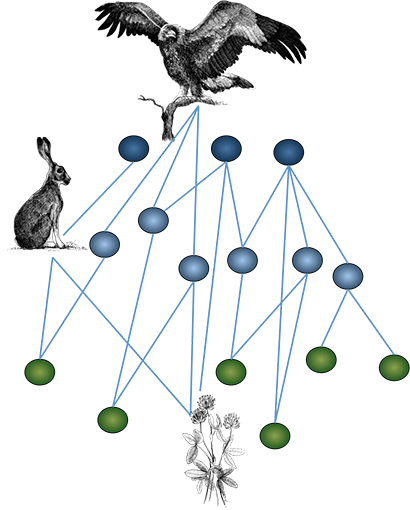
\includegraphics[width=.3\textwidth]{\figeco/ecological-networks-and-community-ecology50}
    $$
   \end{tabular}
   &
   \begin{tabular}{p{.45\textwidth}}
    $$
    \includegraphics[width=.45\textwidth]{\figeco/FaR12-Nature-Fig3a}
    $$
   \end{tabular}
  \end{tabular}
}

%==================================================================
\frame{\frametitle{Two different situations}

  \paragraph{Interactions are not-observed.} 
  \begin{itemize}
   \item Species abundance or presence/absence data (co-occurrence 'networks')
   \item Deep sequencing, metagenomics
  \end{itemize}
  \ra Reconstruct the 'interaction' network \ra \emphase{Lecture 1}

  \bigskip \bigskip 
  \paragraph{Interactions are observed.} 
  \begin{itemize}
   \item Interaction networks, contact networks
   \item Trophic networks, plant-pollinators networks
  \end{itemize}
  \ra Understand the organization/functioning  of the network \ra \emphase{Lecture 2}


}

%==================================================================
\frame{\frametitle{Network reconstruction}

  \paragraph{Generic problem:} $n$ sites, $p$ species, $d$ covariates
  
\pause \hspace{-0.06\textwidth}
\begin{tabular}{c|c|l}
  \onslide+<2->{\paragraph{Abundances:} $Y = n \times p$}
  & 
  \onslide+<3->{\paragraph{Covariates:} $X = n \times d$}
  & 
  \onslide+<4>{\paragraph{Network:} $G = p \times p$ }
  \\
  \hspace{-.02\textwidth} 
  \begin{tabular}{p{.28\textwidth}}
    \onslide+<2->{\begin{tabular}{rrr}
      {\sl Hi.pl} & {\sl An.lu} & {\sl Me.ae} 
      %\footnote{{\sl Hi.pl}: Long rough dab, {\sl An.lu}: Atlantic wolffish, {\sl Me.ae}: Haddock} 
      \\ 
%       Dab & Wolffish & Haddock \\ 
      \hline
      31  &   0  & 108 \\
       4  &   0  & 110 \\
      27  &   0  & 788 \\
      13  &   0  & 295 \\
      23  &   0  &  13 \\
      20  &   0  &  97 \\
      \vdots & \vdots & \vdots 
    \end{tabular}} 
  \end{tabular}
  & 
  \begin{tabular}{p{.3\textwidth}}
    \onslide+<3->{\begin{tabular}{rrr}
      Lat. & Long. & Depth \\ \hline
      71.10 & 22.43 & 349 \\
      71.32 & 23.68 & 382 \\
      71.60 & 24.90 & 294 \\
      71.27 & 25.88 & 304 \\
      71.52 & 28.12 & 384 \\
      71.48 & 29.10 & 344 \\
      \vdots & \vdots & \vdots 
    \end{tabular}} 
  \end{tabular}
  & 
  \hspace{-.02\textwidth} \pause
  \begin{tabular}{p{.3\textwidth}}
    \onslide+<4>{\hspace{-.1\textwidth} 
      \begin{tabular}{c}
        \includegraphics[width=.35\textwidth]{\figCMR/network_BarentsFish_Gfull_full60edges}
      \end{tabular}}
  \end{tabular}
\end{tabular}
  
\begin{itemize}
\item sites could be dates, positions along a gradient
\item 'abundances' could be presence/absence, read counts, etc..
\end{itemize}

\bigskip 
\onslide+<4>{\paragraph{Goal:} infer $G$ based on $X$ and $Y$.}
}

%==================================================================
\frame{\frametitle{Not an easy task}

  \paragraph{A huge search space:}
  $$
  \includegraphics[trim=50 50 0 75, height=.5\textheight, clip]{\fignet/NbGraphs}
  $$
  Number of \textcolor{darkgreen}{undirected graphs} ($2^{p(p-1)/2}$), \textcolor{red}{directed acyclic graphs} (no close form), \textcolor{blue}{spanning trees} ($p^{p-2}$)
}

\section{A brief introduction to graphical models} %==================================================================
\frame{\frametitle{Graphical models} 

  \bigskip
  \paragraph{'Interaction':} 
  need for a probabilistic / statistical counterpart for this concept

  \bigskip 
  \paragraph{Translation:} 
  $$
  \text{species interactions} 
  := 
  \text{dependency structure of a set of random variables}
  $$
  
  \pause\bigskip
  \begin{tabular}{lll}
    \paragraph{Graphical models:} &
    \paragraph{Directed models.} ~ &
    \paragraph{Undirected models.} ~ \\
    \begin{tabular}{p{0.3\textwidth}} A generic \\ framework \\ \refer{Lau96,WaJ08} \end{tabular}
    & 
    \begin{tabular}{p{0.3\textwidth}}   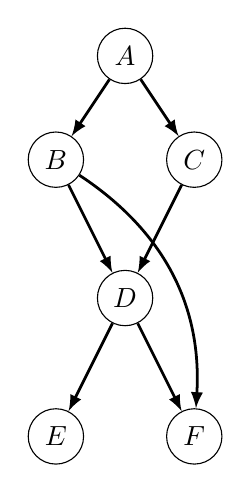
\begin{tikzpicture}
    \node[observed] (a) at (.5*\edgeunit, 2.75*\edgeunit) {$A$};
  \node[observed] (b) at (0*\edgeunit, 2*\edgeunit) {$B$};
  \node[observed] (c) at (1*\edgeunit, 2*\edgeunit) {$C$};
  \node[observed] (d) at (0.5*\edgeunit, 1*\edgeunit) {$D$};
  \node[observed] (e) at (0*\edgeunit, 0*\edgeunit) {$E$};
  \node[observed] (f) at (1*\edgeunit, 0*\edgeunit) {$F$};

  
  \draw[arrow] (a) to (b);  \draw[arrow] (a) to (c);
  \draw[arrow] (b) to (d);  \draw[arrowbendleft] (b) to (f);
  \draw[arrow] (c) to (d);  \draw[arrow] (d) to (e);
  \draw[arrow] (d) to (f);  
  \end{tikzpicture}
 \end{tabular}
    & 
    \begin{tabular}{p{0.3\textwidth}}   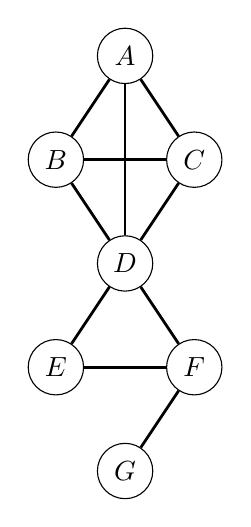
\begin{tikzpicture}
  %   \node[observed] (a) at (0.75*\edgeunit, 1.5*\edgeunit) {$A$};
%   \node[observed] (b) at (0*\edgeunit, 0.75*\edgeunit) {$B$};
%   \node[observed] (c) at (0.75*\edgeunit, 0*\edgeunit) {$C$};
%   \node[observed] (d) at (1.5*\edgeunit, 0.75*\edgeunit) {$D$};
%   \node[observed] (e) at (2.25*\edgeunit, 0*\edgeunit) {$E$};
%   \node[observed] (f) at (3*\edgeunit, 0.75*\edgeunit) {$F$};
%   \node[observed] (g) at (2.25*\edgeunit, 1.5*\edgeunit) {$G$};

  \node[observed] (a) at (.5*\edgeunit, 3*\edgeunit) {$A$};
  \node[observed] (b) at (0*\edgeunit, 2.25*\edgeunit) {$B$};
  \node[observed] (c) at (1*\edgeunit, 2.25*\edgeunit) {$C$};
  \node[observed] (d) at (0.5*\edgeunit, 1.5*\edgeunit) {$D$};
  \node[observed] (e) at (0*\edgeunit, .75*\edgeunit) {$E$};
  \node[observed] (f) at (1*\edgeunit, .75*\edgeunit) {$F$};
  \node[observed] (g) at (.5*\edgeunit, 0*\edgeunit) {$G$};

  
  \draw[edge] (a) to (b);  \draw[edge] (a) to (c);  \draw[edge] (a) to (d);
  \draw[edge] (b) to (c);  \draw[edge] (b) to (d);  \draw[edge] (c) to (d);
  \draw[edge] (d) to (e);  \draw[edge] (d) to (f);  \draw[edge] (e) to (f);
  \draw[edge] (f) to (g);  
  \end{tikzpicture}

 \end{tabular}
    \end{tabular}
  }

%==================================================================
\subsection*{Directed graphical models}
%==================================================================
\frame{\frametitle{Directed graphs = Bayesian networks}

  \paragraph{Definition.} Let $D$ be a {\sl directed acyclic graph} (\emphase{DAG}), the distribution $p$ is said to factorize in $D$ iff
  $$
  p(x_1, \dots x_n) = \prod_{i=1}^n p(x_i \mid x_{pa_D(i)})
  $$
  where $pa_D(i)$ stands for the set of parents of $i$ in $D$.

  \bigskip \pause
  \begin{tabular}{cc}
    \begin{tabular}{c}
    $  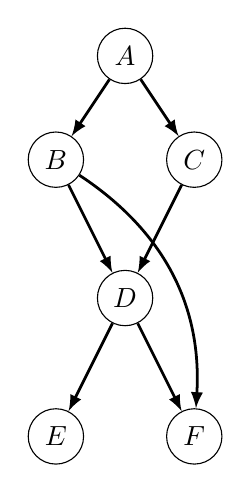
\begin{tikzpicture}
    \node[observed] (a) at (.5*\edgeunit, 2.75*\edgeunit) {$A$};
  \node[observed] (b) at (0*\edgeunit, 2*\edgeunit) {$B$};
  \node[observed] (c) at (1*\edgeunit, 2*\edgeunit) {$C$};
  \node[observed] (d) at (0.5*\edgeunit, 1*\edgeunit) {$D$};
  \node[observed] (e) at (0*\edgeunit, 0*\edgeunit) {$E$};
  \node[observed] (f) at (1*\edgeunit, 0*\edgeunit) {$F$};

  
  \draw[arrow] (a) to (b);  \draw[arrow] (a) to (c);
  \draw[arrow] (b) to (d);  \draw[arrowbendleft] (b) to (f);
  \draw[arrow] (c) to (d);  \draw[arrow] (d) to (e);
  \draw[arrow] (d) to (f);  
  \end{tikzpicture}
$
    \end{tabular}
    &
    \begin{tabular}{p{.7\textwidth}}
      \begin{eqnarray*}
        pa_D(A) = \emptyset, & & pa_D(D) = \{B, C\}, \qquad \dots  \\
        \\
        p(a, \dots f) & = 
        & p(a) \; p(b \mid a) \; p(c \mid a) \\
        & & p(d \mid b, c) \; p(e \mid d) \\
        & & p(f \mid b, d)
        \end{eqnarray*}
    \end{tabular}
  \end{tabular}
  
  \bigskip
  See \refer{SWA17} for an introduction in ecology
}


%==================================================================
\frame{\frametitle{A simple (interesting) example}

  Consider $D =$
  $$
    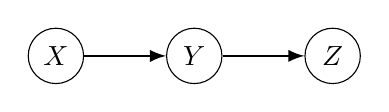
\begin{tikzpicture}
  \node[observed] (x) at (0*\edgeunit, 0*\edgeunit) {$X$};
  \node[observed] (y) at (1*\edgeunit, 0*\edgeunit) {$Y$};
  \node[observed] (z) at (2*\edgeunit, 0*\edgeunit) {$Z$};
  
  \draw[arrow] (x) to (y);  \draw[arrow] (y) to (z);
  \end{tikzpicture}

  $$
  $p(x, y, z)$ is faithful to $D$ iff
  $$
  p(x, y, z) = p(x) \; p(y \mid x) \; p(z \mid y) 
  $$ \pause
  But
  \begin{align*}
   p(x) \; p(y \mid x) \; p(z \mid y) 
%    & = p(x) \; \frac{p(x, y)}{p(x)} \; \frac{p(y, z)}{p(y)} \\
%    & = \frac{p(x, y)}{p(y)} \; \frac{p(y, z)}{p(z)} \; p(z) \\
   & = p(x \mid y) \; p(y \mid z) \; p(z) 
  \end{align*}
  so $p$ is also faithful to $D' =$
  $$
    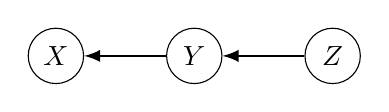
\begin{tikzpicture}
  \node[observed] (x) at (0*\edgeunit, 0*\edgeunit) {$X$};
  \node[observed] (y) at (1*\edgeunit, 0*\edgeunit) {$Y$};
  \node[observed] (z) at (2*\edgeunit, 0*\edgeunit) {$Z$};
  
  \draw[arrow] (z) to (y);  \draw[arrow] (y) to (x);
  \end{tikzpicture}
 
  $$
  \pause and to $D'' =$
  $$
    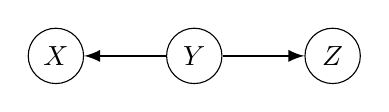
\begin{tikzpicture}
  \node[observed] (x) at (0*\edgeunit, 0*\edgeunit) {$X$};
  \node[observed] (y) at (1*\edgeunit, 0*\edgeunit) {$Y$};
  \node[observed] (z) at (2*\edgeunit, 0*\edgeunit) {$Z$};
  
  \draw[arrow] (y) to (z);  \draw[arrow] (y) to (x);
  \end{tikzpicture}

  $$
  
  \bigskip \pause
  \paragraph{Conclusions.} 
  \begin{itemize}
   \item $p(x)$ is not enough to retrieve the edge orientations
   \item No causal interpretation (causality not addressed here, see \refer{Pea09,Pea09b})
  \end{itemize}
}
  
%==================================================================
\frame{\frametitle{A nice case: Dynamic 'Bayesian' networks (DBN)}

  \paragraph{Temporal data:} $A_t =$ abundance of species $A$ at time $t$
  
  \bigskip
  \begin{tabular}{p{.48\textwidth}p{.48\textwidth}}
  \paragraph{Genuine graphical model.} A DAG: &
  \paragraph{Usual representation.}  \\ 
  $$
  \renewcommand{\nodesize}{2em}
    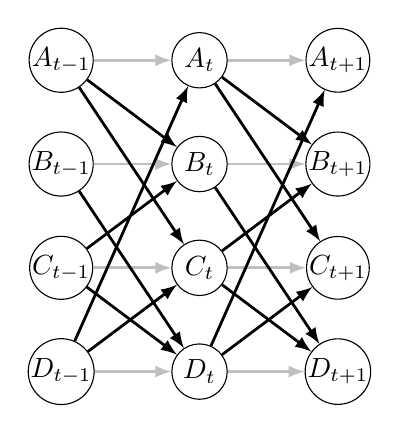
\begin{tikzpicture}
  \node[observed] (a1) at (0*\edgeunit, 2.25*\edgeunit) {$A_{t-1}$};
  \node[observed] (b1) at (0*\edgeunit, 1.5*\edgeunit) {$B_{t-1}$};
  \node[observed] (c1) at (0*\edgeunit, .75*\edgeunit) {$C_{t-1}$};
  \node[observed] (d1) at (0*\edgeunit, 0*\edgeunit) {$D_{t-1}$};
  \node[observed] (a2) at (1*\edgeunit, 2.25*\edgeunit) {$A_t$};
  \node[observed] (b2) at (1*\edgeunit, 1.5*\edgeunit) {$B_t$};
  \node[observed] (c2) at (1*\edgeunit, 0.75*\edgeunit) {$C_t$};
  \node[observed] (d2) at (1*\edgeunit, 0*\edgeunit) {$D_t$};
  \node[observed] (a3) at (2*\edgeunit, 2.25*\edgeunit) {$A_{t+1}$};
  \node[observed] (b3) at (2*\edgeunit, 1.5*\edgeunit) {$B_{t+1}$};
  \node[observed] (c3) at (2*\edgeunit, 0.75*\edgeunit) {$C_{t+1}$};
  \node[observed] (d3) at (2*\edgeunit, 0*\edgeunit) {$D_{t+1}$};
  
  \draw[lightarrow] (a1) to (a2);  \draw[lightarrow] (b1) to (b2);
  \draw[lightarrow] (c1) to (c2);  \draw[lightarrow] (d1) to (d2);
  \draw[lightarrow] (a2) to (a3);  \draw[lightarrow] (b2) to (b3);
  \draw[lightarrow] (c2) to (c3);  \draw[lightarrow] (d2) to (d3);

  \draw[arrow] (a1) to (b2);  \draw[arrow] (a1) to (c2);
  \draw[arrow] (b1) to (d2);  
  \draw[arrow] (c1) to (b2);  \draw[arrow] (c1) to (d2);
  \draw[arrow] (d1) to (c2);  \draw[arrow] (d1) to (a2);  

  \draw[arrow] (a2) to (b3);  \draw[arrow] (a2) to (c3);
  \draw[arrow] (b2) to (d3);  
  \draw[arrow] (c2) to (b3);  \draw[arrow] (c2) to (d3);
  \draw[arrow] (d2) to (c3);  \draw[arrow] (d2) to (a3);  
  \end{tikzpicture}

  \renewcommand{\nodesize}{\commonnodesize}
  $$
  &
  $$
  \renewcommand{\nodesize}{2em}
    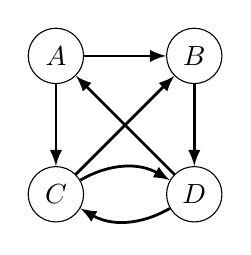
\begin{tikzpicture}
  \node[observed] (a) at (0*\edgeunit, 1*\edgeunit) {$A$};
  \node[observed] (b) at (1*\edgeunit, 1*\edgeunit) {$B$};
  \node[observed] (c) at (0*\edgeunit, 0*\edgeunit) {$C$};
  \node[observed] (d) at (1*\edgeunit, 0*\edgeunit) {$D$};
  
  \draw[arrow] (a) to (b);  \draw[arrow] (a) to (c);
  \draw[arrow] (b) to (d);  
  \draw[arrow] (c) to (b);  \draw[arrowbendleft] (c) to (d);
  \draw[arrowbendleft] (d) to (c);  \draw[arrow] (d) to (a);  
  
  \end{tikzpicture}

  \renewcommand{\nodesize}{\commonnodesize}
  $$
  (not a DAG)
  \end{tabular}
  
  \paragraph{Simpler reconstruction problem:} 
  Find the parents of each species $A$, $B$, ... \emphase{independently}
}


%==================================================================
\subsection*{Undirected graphical models}
%==================================================================
\frame{\frametitle{Undirected graphs = Markov random fields}

  \paragraph{Definition.} Let $G$ be an {\sl undirected graph}, the distribution $p$ is said to factorize in $G$ iff
  $$
  p(x_1, \dots x_n) \propto \prod_{C \in \Ccal(G)} \psi_C(x_C).
  $$
  where $\Ccal(G)$ is the set of maximal cliques of $G$

  \bigskip \bigskip \pause
  \begin{tabular}{cc}
    \begin{tabular}{c}
    $  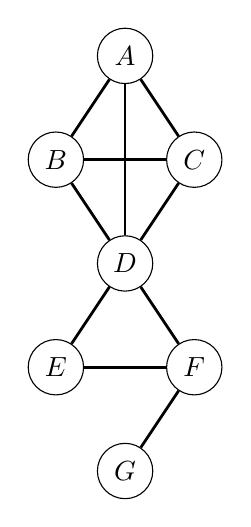
\begin{tikzpicture}
  %   \node[observed] (a) at (0.75*\edgeunit, 1.5*\edgeunit) {$A$};
%   \node[observed] (b) at (0*\edgeunit, 0.75*\edgeunit) {$B$};
%   \node[observed] (c) at (0.75*\edgeunit, 0*\edgeunit) {$C$};
%   \node[observed] (d) at (1.5*\edgeunit, 0.75*\edgeunit) {$D$};
%   \node[observed] (e) at (2.25*\edgeunit, 0*\edgeunit) {$E$};
%   \node[observed] (f) at (3*\edgeunit, 0.75*\edgeunit) {$F$};
%   \node[observed] (g) at (2.25*\edgeunit, 1.5*\edgeunit) {$G$};

  \node[observed] (a) at (.5*\edgeunit, 3*\edgeunit) {$A$};
  \node[observed] (b) at (0*\edgeunit, 2.25*\edgeunit) {$B$};
  \node[observed] (c) at (1*\edgeunit, 2.25*\edgeunit) {$C$};
  \node[observed] (d) at (0.5*\edgeunit, 1.5*\edgeunit) {$D$};
  \node[observed] (e) at (0*\edgeunit, .75*\edgeunit) {$E$};
  \node[observed] (f) at (1*\edgeunit, .75*\edgeunit) {$F$};
  \node[observed] (g) at (.5*\edgeunit, 0*\edgeunit) {$G$};

  
  \draw[edge] (a) to (b);  \draw[edge] (a) to (c);  \draw[edge] (a) to (d);
  \draw[edge] (b) to (c);  \draw[edge] (b) to (d);  \draw[edge] (c) to (d);
  \draw[edge] (d) to (e);  \draw[edge] (d) to (f);  \draw[edge] (e) to (f);
  \draw[edge] (f) to (g);  
  \end{tikzpicture}

$
    \end{tabular}
    &
    \begin{tabular}{p{.7\textwidth}}
      \begin{eqnarray*}
%         p(a, \dots g) & \propto 
%         & \psi_1(a, b, c) \; \psi_2(a, b, d) \; \psi_3(a, c, d) \; \psi_4(b, c, d) \\
%         & & \psi_5(d, e, f) \; \psi_6(f, g) \\\pause
%       \text{but also} \qquad \\
        p(a, \dots g) & \propto 
        & \psi_1(a, b, c, d) \\
        & & \psi_2(d, e, f) \; \psi_3(f, g) 
      \end{eqnarray*}
%       \ra Only consider \emphase{maximal} cliques
    \end{tabular}
  \end{tabular}
}

%====================================================================
\frame{\frametitle{Conditional independence}

  \paragraph{Property.} If $p(x) > 0$, 
  $$
  \text{separation} \qquad \Leftrightarrow \qquad \text{conditional independence}
  $$

  \bigskip \pause
  \begin{tabular}{ccc}
    \hspace{.2\textwidth} 
    &
    \begin{tabular}{c}
    $  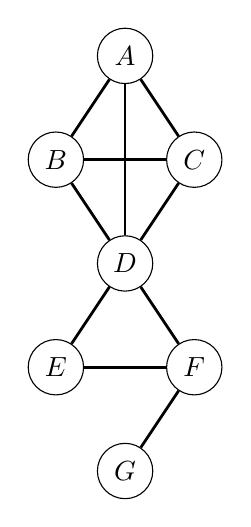
\begin{tikzpicture}
  %   \node[observed] (a) at (0.75*\edgeunit, 1.5*\edgeunit) {$A$};
%   \node[observed] (b) at (0*\edgeunit, 0.75*\edgeunit) {$B$};
%   \node[observed] (c) at (0.75*\edgeunit, 0*\edgeunit) {$C$};
%   \node[observed] (d) at (1.5*\edgeunit, 0.75*\edgeunit) {$D$};
%   \node[observed] (e) at (2.25*\edgeunit, 0*\edgeunit) {$E$};
%   \node[observed] (f) at (3*\edgeunit, 0.75*\edgeunit) {$F$};
%   \node[observed] (g) at (2.25*\edgeunit, 1.5*\edgeunit) {$G$};

  \node[observed] (a) at (.5*\edgeunit, 3*\edgeunit) {$A$};
  \node[observed] (b) at (0*\edgeunit, 2.25*\edgeunit) {$B$};
  \node[observed] (c) at (1*\edgeunit, 2.25*\edgeunit) {$C$};
  \node[observed] (d) at (0.5*\edgeunit, 1.5*\edgeunit) {$D$};
  \node[observed] (e) at (0*\edgeunit, .75*\edgeunit) {$E$};
  \node[observed] (f) at (1*\edgeunit, .75*\edgeunit) {$F$};
  \node[observed] (g) at (.5*\edgeunit, 0*\edgeunit) {$G$};

  
  \draw[edge] (a) to (b);  \draw[edge] (a) to (c);  \draw[edge] (a) to (d);
  \draw[edge] (b) to (c);  \draw[edge] (b) to (d);  \draw[edge] (c) to (d);
  \draw[edge] (d) to (e);  \draw[edge] (d) to (f);  \draw[edge] (e) to (f);
  \draw[edge] (f) to (g);  
  \end{tikzpicture}

$
    \end{tabular}
    &
    \begin{tabular}{p{.7\textwidth}}
    \begin{itemize}
     \item $A \not\independent B$ \\ ~
     \item $A \not\independent D \mid B$ \\ ~
     \item $A \independent D \mid \{B, C\}$ \\ ~
     \item $\{A, B, C\} \independent \{E, F, G\} \mid D$ \\ ~
     \item $\{B, C\} \independent \{E, F\} \mid D$ \\ ~
    \end{itemize}
    \end{tabular}
  \end{tabular}

}
  
%====================================================================
\subsection*{Missing actors}
%====================================================================
\frame{\frametitle{Missing 'actors'}

  \paragraph{Incomplete observations.} Most of the time, not all actors (species, environmental covariate, ...) are observed
  
  \bigskip \bigskip 
  \paragraph{Missing variable = marginalisation.} 
  \begin{center}
  \begin{tabular}{ccccc}
    $B \independent C \mid A$ & & $A$ missing & & $B \not\independent C$ \\
    \begin{tabular}{c}
    $  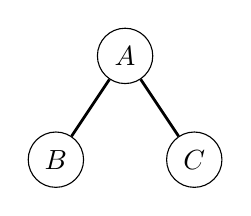
\begin{tikzpicture}
    \node[observed] (a) at (.5*\edgeunit, 0.75*\edgeunit) {$A$};
  \node[observed] (b) at (0*\edgeunit, 0*\edgeunit) {$B$};
  \node[observed] (c) at (1*\edgeunit, 0*\edgeunit) {$C$};

  
  \draw[edge] (a) to (b);  \draw[edge] (a) to (c);
  \end{tikzpicture}
$
    \end{tabular}
    & \qquad \qquad &
    \begin{tabular}{c}
    $  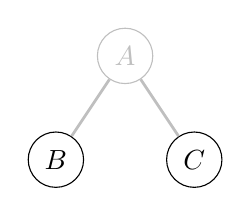
\begin{tikzpicture}
    \node[eliminated] (a) at (.5*\edgeunit, 0.75*\edgeunit) {$A$};
  \node[observed] (b) at (0*\edgeunit, 0*\edgeunit) {$B$};
  \node[observed] (c) at (1*\edgeunit, 0*\edgeunit) {$C$};

  
  \draw[lightedge] (a) to (b);  \draw[lightedge] (a) to (c);
  \end{tikzpicture}
$
    \end{tabular}
    & \qquad \qquad &
    \begin{tabular}{c}
    $  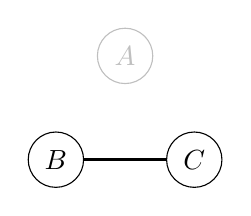
\begin{tikzpicture}
    \node[eliminated] (a) at (.5*\edgeunit, 0.75*\edgeunit) {$A$};
  \node[observed] (b) at (0*\edgeunit, 0*\edgeunit) {$B$};
  \node[observed] (c) at (1*\edgeunit, 0*\edgeunit) {$C$};

  
  \draw[edge] (b) to (c);
  \end{tikzpicture}
$
    \end{tabular}
  \end{tabular}
  \end{center}
  
  \bigskip
  \paragraph{Indeed:}
  $$
  p(a, b, c) = p(a) p(b \mid a) p(c \mid a)
  $$
  but $A$ is not observed, so only $p(b, c)$ can be considered:
  $$
  p(b, c) = \sum_a p(a, b, c) = \sum_a p(\emphase{a}) p(b \mid \emphase{a}) p(c \mid \emphase{a}) \neq p(b) p(c)
  $$
}

%====================================================================
\frame{\frametitle{'Spurious' edges}

  Possibly dramatic effect on the observable dependency structure:
  \begin{center}
  \begin{tabular}{ccccc}
    'Truth' && $C$ missing && $D$ missing \\
    \begin{tabular}{c}
    $  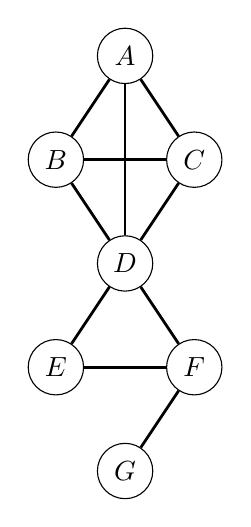
\begin{tikzpicture}
  %   \node[observed] (a) at (0.75*\edgeunit, 1.5*\edgeunit) {$A$};
%   \node[observed] (b) at (0*\edgeunit, 0.75*\edgeunit) {$B$};
%   \node[observed] (c) at (0.75*\edgeunit, 0*\edgeunit) {$C$};
%   \node[observed] (d) at (1.5*\edgeunit, 0.75*\edgeunit) {$D$};
%   \node[observed] (e) at (2.25*\edgeunit, 0*\edgeunit) {$E$};
%   \node[observed] (f) at (3*\edgeunit, 0.75*\edgeunit) {$F$};
%   \node[observed] (g) at (2.25*\edgeunit, 1.5*\edgeunit) {$G$};

  \node[observed] (a) at (.5*\edgeunit, 3*\edgeunit) {$A$};
  \node[observed] (b) at (0*\edgeunit, 2.25*\edgeunit) {$B$};
  \node[observed] (c) at (1*\edgeunit, 2.25*\edgeunit) {$C$};
  \node[observed] (d) at (0.5*\edgeunit, 1.5*\edgeunit) {$D$};
  \node[observed] (e) at (0*\edgeunit, .75*\edgeunit) {$E$};
  \node[observed] (f) at (1*\edgeunit, .75*\edgeunit) {$F$};
  \node[observed] (g) at (.5*\edgeunit, 0*\edgeunit) {$G$};

  
  \draw[edge] (a) to (b);  \draw[edge] (a) to (c);  \draw[edge] (a) to (d);
  \draw[edge] (b) to (c);  \draw[edge] (b) to (d);  \draw[edge] (c) to (d);
  \draw[edge] (d) to (e);  \draw[edge] (d) to (f);  \draw[edge] (e) to (f);
  \draw[edge] (f) to (g);  
  \end{tikzpicture}

$
    \end{tabular}
    & \qquad \qquad &
    \begin{tabular}{c}
    $  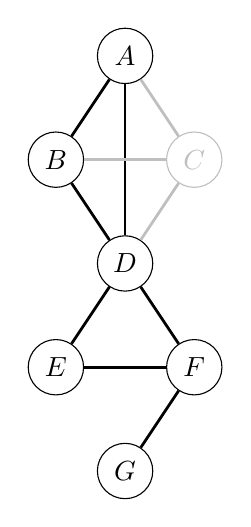
\begin{tikzpicture}
  %   \node[observed] (a) at (0.75*\edgeunit, 1.5*\edgeunit) {$A$};
%   \node[observed] (b) at (0*\edgeunit, 0.75*\edgeunit) {$B$};
%   \node[observed] (c) at (0.75*\edgeunit, 0*\edgeunit) {$C$};
%   \node[observed] (d) at (1.5*\edgeunit, 0.75*\edgeunit) {$D$};
%   \node[observed] (e) at (2.25*\edgeunit, 0*\edgeunit) {$E$};
%   \node[observed] (f) at (3*\edgeunit, 0.75*\edgeunit) {$F$};
%   \node[observed] (g) at (2.25*\edgeunit, 1.5*\edgeunit) {$G$};

  \node[observed] (a) at (.5*\edgeunit, 3*\edgeunit) {$A$};
  \node[observed] (b) at (0*\edgeunit, 2.25*\edgeunit) {$B$};
  \node[eliminated] (c) at (1*\edgeunit, 2.25*\edgeunit) {$C$};
  \node[observed] (d) at (0.5*\edgeunit, 1.5*\edgeunit) {$D$};
  \node[observed] (e) at (0*\edgeunit, .75*\edgeunit) {$E$};
  \node[observed] (f) at (1*\edgeunit, .75*\edgeunit) {$F$};
  \node[observed] (g) at (.5*\edgeunit, 0*\edgeunit) {$G$};

  
  \draw[edge] (a) to (b);  \draw[lightedge] (a) to (c);  \draw[edge] (a) to (d);
  \draw[lightedge] (b) to (c);  \draw[edge] (b) to (d);  \draw[lightedge] (c) to (d);
  \draw[edge] (d) to (e);  \draw[edge] (d) to (f);  \draw[edge] (e) to (f);
  \draw[edge] (f) to (g);  
  \end{tikzpicture}
$
    \end{tabular}
    & \qquad \qquad &
    \begin{tabular}{c}
    $  \begin{tikzpicture}
  %   \node[observed] (a) at (0.75*\edgeunit, 1.5*\edgeunit) {$A$};
%   \node[observed] (b) at (0*\edgeunit, 0.75*\edgeunit) {$B$};
%   \node[observed] (c) at (0.75*\edgeunit, 0*\edgeunit) {$C$};
%   \node[observed] (d) at (1.5*\edgeunit, 0.75*\edgeunit) {$D$};
%   \node[observed] (e) at (2.25*\edgeunit, 0*\edgeunit) {$E$};
%   \node[observed] (f) at (3*\edgeunit, 0.75*\edgeunit) {$F$};
%   \node[observed] (g) at (2.25*\edgeunit, 1.5*\edgeunit) {$G$};

  \node[observed] (a) at (.5*\edgeunit, 3*\edgeunit) {$A$};
  \node[observed] (b) at (0*\edgeunit, 2.25*\edgeunit) {$B$};
  \node[observed] (c) at (1*\edgeunit, 2.25*\edgeunit) {$C$};
  \node[eliminated] (d) at (0.5*\edgeunit, 1.5*\edgeunit) {$D$};
  \node[observed] (e) at (0*\edgeunit, .75*\edgeunit) {$E$};
  \node[observed] (f) at (1*\edgeunit, .75*\edgeunit) {$F$};
  \node[observed] (g) at (.5*\edgeunit, 0*\edgeunit) {$G$};

  
  \draw[edge] (a) to (b);  \draw[edge] (a) to (c);  \draw[lightedge] (a) to (d);
  \draw[edge] (b) to (c);  \draw[lightedge] (b) to (d);  \draw[lightedge] (c) to (d);
  \draw[lightedge] (d) to (e);  \draw[lightedge] (d) to (f);  \draw[edge] (e) to (f);
  \draw[edge] (f) to (g);  

  \draw[edgered] (a) to (e);  \draw[edgered] (b) to (e);  \draw[edgebendrightred] (c) to (e);    
  \draw[edgered] (a) to (f);  \draw[edgebendleftred] (b) to (f);  \draw[edgered] (c) to (f);  
  \end{tikzpicture}
$
    \end{tabular}
  \end{tabular}
  \end{center}
  
  \ra Need to account for 'all' available information

}



\section{Network inference} %==================================================================
\subsection*{Latent GGM}
\frame{\frametitle{Back to ecology}

}

%==================================================================
\frame{\frametitle{Poisson log-normal model}

  \paragraph{Data:} $n$ independent sites (no spatial structure), $p$ species, 
  $$
  Y_{ij} = \text{ abundance of species $j$ in site $i$}
  $$
  
  \bigskip \pause
  \paragraph{Poisson log-normal (PLN) model \refer{AiH89}:} 
  \begin{itemize}
   \item For each site, draw independently
   $$
   Z_i \sim \Ncal_p(0, \Omega^{-1})
   $$
   \item \pause For each species in each site, draw independently (given $Z$)
   $$
   Y_{ij} \sim \Pcal(\exp(\mu_j + Z_{ij}))
   $$
  \end{itemize} \pause
  summarized as
  $$
  \{Y_i\} \text{ iid} \sim PLN(\mu, \Omega^{-1})
  $$

  \bigskip \pause
  \paragraph{Interpretation.}
  \begin{itemize}
%   \item PLN is a mixed model
  \item $\mu_j =$ mean (log-)abundance of species $j$
  \item $\Omega = $ dependency structure (encoded in the latent layer)
  \end{itemize}
}

%==================================================================
\frame{\frametitle{PLNnetworks}

  \paragraph{PLN network model.} Same model as PLN + sparsity assumption:
  $$
  \{Y_i\} \text{ iid} \sim PLN(\mu, \Omega)
  \qquad \qquad + \emphase{\Omega \text{ sparse}}
  $$
  
  \bigskip \bigskip \pause
  \paragraph{Inference algorithm.} Variational EM + sparsity inducing norm \refer{CMR18,CMR19}:
  $$
  \max_{\mu, \Omega} \widetilde{\log p}(Y; \mu, \Omega) - \lambda \sum_{j < k} |\omega_{jk}|
  $$
  \ra Alternate convex problems \\
  \ra Fast solution ({\tt PLNmodels} R package)
  
  \bigskip
  \begin{itemize}
   \item Resampling (StARS \refer{LRW10}) is highly recommended for robustness
  \end{itemize}
}

%==================================================================
\frame{\frametitle{Modeling limitation}

  \paragraph{All latent (GGM) models} infer the dependency struture of the latent $Z$, not of the observed abundances $Y$
  
  \bigskip \bigskip 
  \renewcommand{\nodesize}{2em}
  \begin{overprint}
    \onslide<2>
    $$
    \begin{array}{ccc}
    p(Z, Y) & & p(Y) \\ ~\\
      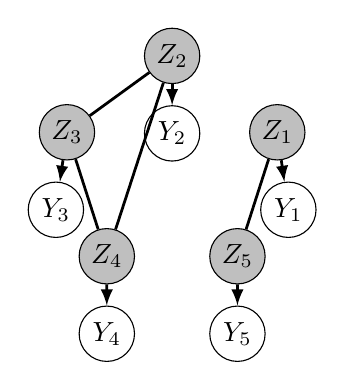
\begin{tikzpicture}[scale=.8]
  \node[hidden] (Z1) at ( 0.95*\edgeunit,  0.31*\edgeunit) {$Z_1$};
  \node[hidden] (Z2) at (-0.00*\edgeunit,  1.00*\edgeunit) {$Z_2$};
  \node[hidden] (Z3) at (-0.95*\edgeunit,  0.31*\edgeunit) {$Z_3$};
  \node[hidden] (Z4) at (-0.59*\edgeunit, -0.81*\edgeunit) {$Z_4$};
  \node[hidden] (Z5) at ( 0.59*\edgeunit, -0.81*\edgeunit) {$Z_5$};
  
  \draw[edge] (Z1) to (Z5);  \draw[edge] (Z2) to (Z3);  
  \draw[edge] (Z2) to (Z4);  \draw[edge] (Z3) to (Z4); 

  \node[observed] (Y1) at ( 1.05*\edgeunit, -0.39*\edgeunit) {$Y_1$};
  \node[observed] (Y2) at (-0.00*\edgeunit,  0.30*\edgeunit) {$Y_2$};
  \node[observed] (Y3) at (-1.05*\edgeunit, -0.39*\edgeunit) {$Y_3$};
  \node[observed] (Y4) at (-0.59*\edgeunit, -1.51*\edgeunit) {$Y_4$};
  \node[observed] (Y5) at ( 0.59*\edgeunit, -1.51*\edgeunit) {$Y_5$};
  
  \draw[arrow] (Z1) to (Y1); 
  \draw[arrow] (Z2) to (Y2);
  \draw[arrow] (Z3) to (Y3);
  \draw[arrow] (Z4) to (Y4);
  \draw[arrow] (Z5) to (Y5);
  \end{tikzpicture}

    & \qquad \qquad &
      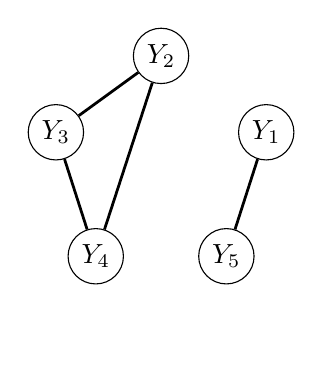
\begin{tikzpicture}[scale=.8]
  \node[observed] (Y1) at ( 0.95*\edgeunit,  0.31*\edgeunit) {$Y_1$};
  \node[observed] (Y2) at (-0.00*\edgeunit,  1.00*\edgeunit) {$Y_2$};
  \node[observed] (Y3) at (-0.95*\edgeunit,  0.31*\edgeunit) {$Y_3$};
  \node[observed] (Y4) at (-0.59*\edgeunit, -0.81*\edgeunit) {$Y_4$};
  \node[observed] (Y5) at ( 0.59*\edgeunit, -0.81*\edgeunit) {$Y_5$};
  \node[empty] (YY) at ( 0.59*\edgeunit, -1.51*\edgeunit) {};

  \draw[edge] (Y1) to (Y5);  \draw[edge] (Y2) to (Y3);  
  \draw[edge] (Y2) to (Y4);  \draw[edge] (Y3) to (Y4);  
  
  \end{tikzpicture}

    \end{array}
    $$
    \onslide<3>
    $$
    \begin{array}{ccc}
    p(Z, Y) & & p(Y) \\ ~\\
      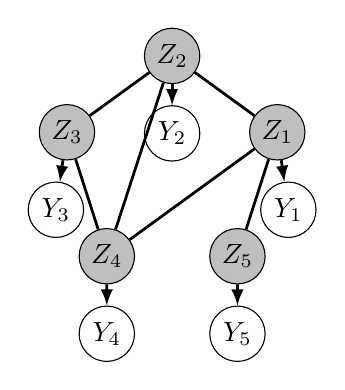
\begin{tikzpicture}[scale=.8]
    \node[hidden] (Z1) at ( 0.95*\edgeunit,  0.31*\edgeunit) {$Z_1$};
    \node[hidden] (Z2) at (-0.00*\edgeunit,  1.00*\edgeunit) {$Z_2$};
    \node[hidden] (Z3) at (-0.95*\edgeunit,  0.31*\edgeunit) {$Z_3$};
    \node[hidden] (Z4) at (-0.59*\edgeunit, -0.81*\edgeunit) {$Z_4$};
    \node[hidden] (Z5) at ( 0.59*\edgeunit, -0.81*\edgeunit) {$Z_5$};
    
    \draw[edge] (Z1) to (Z2);  \draw[edge] (Z1) to (Z4);  
    \draw[edge] (Z1) to (Z5);  \draw[edge] (Z2) to (Z3);  
    \draw[edge] (Z2) to (Z4);  \draw[edge] (Z3) to (Z4); 

    \node[observed] (Y1) at ( 1.05*\edgeunit, -0.39*\edgeunit) {$Y_1$};
    \node[observed] (Y2) at (-0.00*\edgeunit,  0.30*\edgeunit) {$Y_2$};
    \node[observed] (Y3) at (-1.05*\edgeunit, -0.39*\edgeunit) {$Y_3$};
    \node[observed] (Y4) at (-0.59*\edgeunit, -1.51*\edgeunit) {$Y_4$};
    \node[observed] (Y5) at ( 0.59*\edgeunit, -1.51*\edgeunit) {$Y_5$};

    \draw[arrow] (Z1) to (Y1); 
    \draw[arrow] (Z2) to (Y2);
    \draw[arrow] (Z3) to (Y3);
    \draw[arrow] (Z4) to (Y4);
    \draw[arrow] (Z5) to (Y5);
  \end{tikzpicture}

    & \qquad \qquad &
      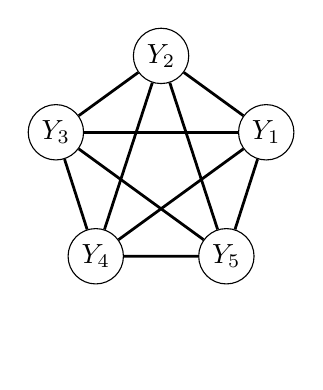
\begin{tikzpicture}[scale=.8]
  \node[observed] (Y1) at ( 0.95*\edgeunit,  0.31*\edgeunit) {$Y_1$};
  \node[observed] (Y2) at (-0.00*\edgeunit,  1.00*\edgeunit) {$Y_2$};
  \node[observed] (Y3) at (-0.95*\edgeunit,  0.31*\edgeunit) {$Y_3$};
  \node[observed] (Y4) at (-0.59*\edgeunit, -0.81*\edgeunit) {$Y_4$};
  \node[observed] (Y5) at ( 0.59*\edgeunit, -0.81*\edgeunit) {$Y_5$};
  \node[empty] (YY) at ( 0.59*\edgeunit, -1.51*\edgeunit) {};

  \draw[edge] (Y1) to (Y2);  \draw[edge] (Y1) to (Y3);  
  \draw[edge] (Y1) to (Y4);  \draw[edge] (Y1) to (Y5);  
  \draw[edge] (Y2) to (Y3);  \draw[edge] (Y2) to (Y4); 
  \draw[edge] (Y2) to (Y5);  \draw[edge] (Y3) to (Y4);  
  \draw[edge] (Y3) to (Y5);  \draw[edge] (Y4) to (Y5);  
  \end{tikzpicture}

    \end{array}
    $$
  \end{overprint}
  \renewcommand{\nodesize}{\commonnodesize}
}

%==================================================================
\frame{\frametitle{Illustration}

  \paragraph{Barents fish dataset:} $n = 89$ sites, $p = 30$ species
  
  \bigskip
  \begin{tabular}{p{.45\textwidth}p{.45\textwidth}}
    \begin{tabular}{c}
      \vspace{.04\textheight}
      Regularization path ($\lambda$) \\
      \includegraphics[width=.45\textwidth, height=.45\textheight]{\figbarents/BarentsFish_Gnull_criteria}
    \end{tabular}
    &
%     \hspace{-.1\textwidth}
    \begin{overprint}
      \onslide<2>
        \begin{tabular}{c}
          Covariance ($\widehat{\Sigma}$) \\ 
          \includegraphics[width=.4\textwidth]{\figbarents/BarentsFish_Gnull_sigma}
        \end{tabular}
      \onslide<3>
        \begin{tabular}{c}
          Precision ($\widehat{\Omega}$) \\ 
          \includegraphics[width=.4\textwidth]{\figbarents/BarentsFish_Gnull_omega}
        \end{tabular}
      \onslide<4>
        \begin{tabular}{c}
          Network ($\widehat{G}$) \\ 
          \includegraphics[width=.4\textwidth]{\figbarents/BarentsFish_Gnull_network}
        \end{tabular}
    \end{overprint}
  \end{tabular}

  {\tt PLNnetwork} R package  \refer{CMR19}: \qquad
  {\tt PLNnetwork(Y $\sim$  1)}
}

%==================================================================
\subsection*{Accounting for covariates}
\frame{\frametitle{Accounting for covariates}

  \paragraph{Aim of network inference:} determine which species are 'in direct interaction' \\
  \ra Avoid 'spurious edges'
  
  \hspace{-.05\textwidth}
  \begin{tabular}{p{.45\textwidth}p{.45\textwidth}}
    \begin{tabular}{p{.4\textwidth}}
      \onslide+<2->{
        \paragraph{Environmental variations} may jointly affect species, which do not actually interact \\
        }
      \onslide+<4->{
        \bigskip \bigskip 
        \paragraph{Introducing covariates.} ~ \\
        $x_i =$ vector of covariates for site $i$ \\
        e.g. $x_i = (\text{temperature}, \text{altitude}, ...)$
        }
    \end{tabular}
    &
%     \hspace{-.1\textwidth}
    \begin{tabular}{p{.45\textwidth}}
      \onslide+<3->{
        \includegraphics[width=.4\textwidth]{\figbarents/BarentsFish_Sigmanull_Sigmafull}
        }
    \end{tabular}
  \end{tabular}
  
  \onslide+<4->{
    Add a regression term in the PLN model:
    $$
    Y_{ij} \mid Z_{ij} \sim \Pcal(\exp(\emphase{x_i^\intercal \beta_j} + Z_{ij}))
    $$
    $\beta_j =$ vector of environmental effects on species $j$
    }

}

%====================================================================
\frame{\frametitle{Barents fish} 

  \begin{center}
  \begin{tabular}{lccc}
    & no covariate & \textcolor{blue}{temp. \& depth} & \textcolor{red}{all covariates} \\
    \hline
    \rotatebox{90}{$\qquad\quad\lambda=.20$} &
    \includegraphics[width=.22\textwidth]{\figCMR/network_BarentsFish_Gnull_full60edges} &
    \includegraphics[width=.22\textwidth]{\figCMR/network_BarentsFish_Gsel_full60edges} &
    \includegraphics[width=.22\textwidth]{\figCMR/network_BarentsFish_Gfull_full60edges} 
    \vspace{-0.05\textheight} \\ \hline
    %
    \rotatebox{90}{$\qquad\quad\lambda=.28$} &
    \includegraphics[width=.22\textwidth]{\figCMR/network_BarentsFish_Gnull_sel60edges} & \includegraphics[width=.22\textwidth]{\figCMR/network_BarentsFish_Gsel_sel60edges} &
    \includegraphics[width=.22\textwidth]{\figCMR/network_BarentsFish_Gfull_sel60edges} 
    \vspace{-0.05\textheight} \\ \hline
    %
    \rotatebox{90}{$\qquad\quad\lambda=.84$} &
    \includegraphics[width=.22\textwidth]{\figCMR/network_BarentsFish_Gnull_null60edges} &
    \includegraphics[width=.22\textwidth]{\figCMR/network_BarentsFish_Gsel_null60edges} &
    \includegraphics[width=.22\textwidth]{\figCMR/network_BarentsFish_density} 
%     \includegraphics[width=.22\textwidth]{\figCMR/network_BarentsFish_Gfull_null60edges}  
  \end{tabular}
  \end{center}

}


\section{Temporal data} % \cite{BPG18}: trop long terme

\begin{itemize}
 \item Review \& methods: \cite{FLG15}
 \item Fundamental limitations: \cite{AML17} ('all state variables are measured without any measurement noise')
 \item Actually doable? Steady-state approach: \cite{XAF17}
 \item Lotka-Volterra (simul): \cite{BeW14}
 \item Lotka-Volterra micro: \cite{SBT13}
 \item Pseudo Lotka-Volterra: \cite{AHL12}, \cite{FaR12}
 \item Presence-absence: \cite{SWA17} (data \& code: \url{https://github.com/elsander/PresenceAbsenceNetworks})
 \item Likelihood-free approach (Lotka-Volterra as an example): \cite{TRB17}
\end{itemize}



%******************************************************************************%******************************************************************************
\chapter{Network topology}
\section{Introduction} %==================================================================
\frame{\frametitle{Different types of networks}

  \paragraph{Network =} natural and convenient way to represent ecological 'interactions' \refer{Bas09}

  \bigskip \bigskip \pause
  \paragraph{Many types of networks:} trophic, plant-pollinator, 'interaction'

  \bigskip \bigskip \pause
  \paragraph{Aim:} understand their organisations, i.e. analyse their {\sl topology}
  \begin{overprint}
    \onslide<4>
    \begin{tabular}{p{.35\textwidth}p{.55\textwidth}}
      \begin{tabular}{p{.35\textwidth}}
        Do trophic levels actually exist? \\
        \\
        {\tiny \url{en.wikipedia.org/wiki/Trophic_coherence}}
      \end{tabular}
      &
      \begin{tabular}{p{.55\textwidth}}
        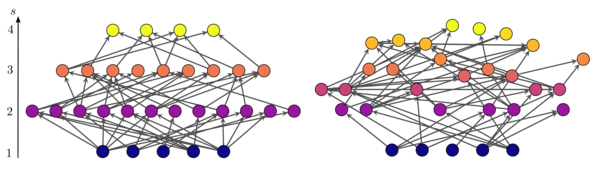
\includegraphics[trim=20 0 300 0, width=.35\textwidth, clip]{\figeco/WikipediaTrophicNetwork} \\
        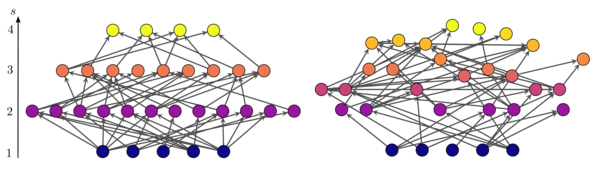
\includegraphics[trim=310 0 0 0, width=.35\textwidth, clip]{\figeco/WikipediaTrophicNetwork} 
      \end{tabular} 
    \end{tabular}
    \onslide<5>
    \begin{tabular}{p{.35\textwidth}p{.55\textwidth}}
      \begin{tabular}{p{.35\textwidth}}
        Generalist vs specialist pollinators?  \\
        \\
        {\tiny \url{seibutsu.biology.kyushu-u.ac.jp/~satake}}
      \end{tabular}
      &
      \begin{tabular}{p{.55\textwidth}}
        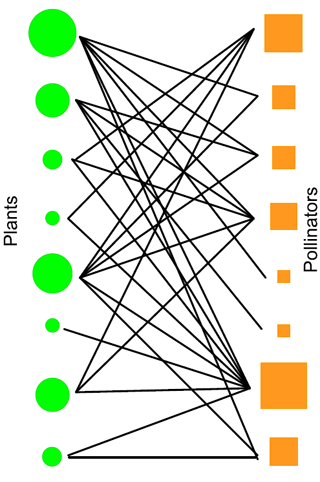
\includegraphics[height=.45\textwidth,angle=270]{\figeco/SatakePlantPollinatorNetwork}
      \end{tabular} 
    \end{tabular}
    \onslide<6>
    \begin{tabular}{p{.35\textwidth}p{.55\textwidth}}
      \begin{tabular}{p{.35\textwidth}}
        Is the network 'organized'? \\
        \\
        If so, how? \\
        \\
        {\tiny \url{www.allisonbarner.com}}
      \end{tabular}
      &
      \begin{tabular}{p{.55\textwidth}}
        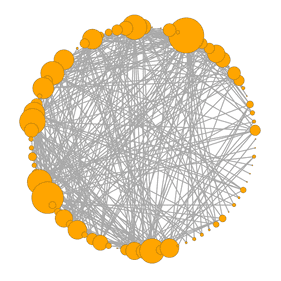
\includegraphics[width=.4\textwidth]{\figeco/BarnerEcologicalNetwork}
      \end{tabular} 
    \end{tabular}
  \end{overprint}
}
  
%==================================================================
\frame{\frametitle{Modelling approach}

  \paragraph{Mathematical counterpart:} 
  $$
  \text{ecological {\sl network}}
  \quad \leftrightarrow \quad
  \text{random {\sl graph}}  
  $$

  \bigskip \pause
  \paragraph{Random graph:}   $n$ nodes  = species, individuals, ... ($1 \leq i, j \leq n$), 
  $$
  Y_{ij} = \text{ 'value' of the edge between node $i$ and $j$}
  $$
  Random graph model = joint distribution of all edge values:
  $$
  p(\{Y_{ij}\}_{i, j})
  \qquad \rightarrow \qquad \simeq n^2 \text{ random variables}
  $$

  \bigskip \bigskip \pause
  \begin{tabular}{p{.35\textwidth}p{.6\textwidth}}
    \paragraph{Type of network:} & \paragraph{Type of edge:} \\ %~ \\
      directed / undirected & $Y_{ij} = Y_{ji}$ or not \\ %~ \\
      binary / valued ('weighted') & $Y_{ij} \in \{0, 1\}$ or $\Rbb$ \\ %~ \\
      multivariate ('multiplex') & $Y_{ij} \in \{0, 1\}^d$ or $\Rbb^d$ \\
      & or $\{0, 1\} \times \{a, b, c, d\} \times \Nbb \times \Rbb$
  \end{tabular}

}

%==================================================================
\frame{\frametitle{A model: what for?}

  Many different aims: \\~
  \begin{enumerate}[($a$)]
    \item \emphase{Mechanistic} model: pretends to encode the process that actually generated the data \\~
    \item \emphase{Empirical} model: enables to simulate data similar to the observed ones \\~ 
    \item \emphase{Null} model: serves as a reference to detect 'unexpected behaviors' 
  \end{enumerate}

  \bigskip \bigskip \pause
  \paragraph{Here,} focus on 
  \begin{itemize}
    \item ($b$) and ($c$): empirical and null models
    \item for binary networks (with some extensions)
  \end{itemize}


}

\section{Some models} %******************************************************************************
\subsection{Degree-based models}

%******************************************************************************
\subsection{Latent-space models}

%******************************************************************************
\subsection{Accounting for covariates}

\section{Block-models} \begin{itemize}
 \item \cite{LDV15}, \cite{MPD14}
\end{itemize}


%******************************************************************************
\subsection{Stochastic block-model (SBM)}

%******************************************************************************
\subsection{Latent block-model (LBM)}

\section{Network motifs} %******************************************************************************
\subsection{A null model}

%******************************************************************************
\subsection{B-motifs}



%******************************************************************************%******************************************************************************
\newpage
{\footnotesize
% \begin{multicols}{2}
\bibliographystyle{/home/robin/LATEX/Biblio/astats}
% \bibliographystyle{plain}
\bibliography{/home/robin/Biblio/BibGene}
% \end{multicols}
}
  
%******************************************************************************
%******************************************************************************
\end{document}
%******************************************************************************
%******************************************************************************
